% Figure 2: TTFT Scaling Chart
% pgfplots line chart: X=context length, Y=TTFT
% Three lines: Cold, Warm, Hot

\begin{figure}[t]
\centering
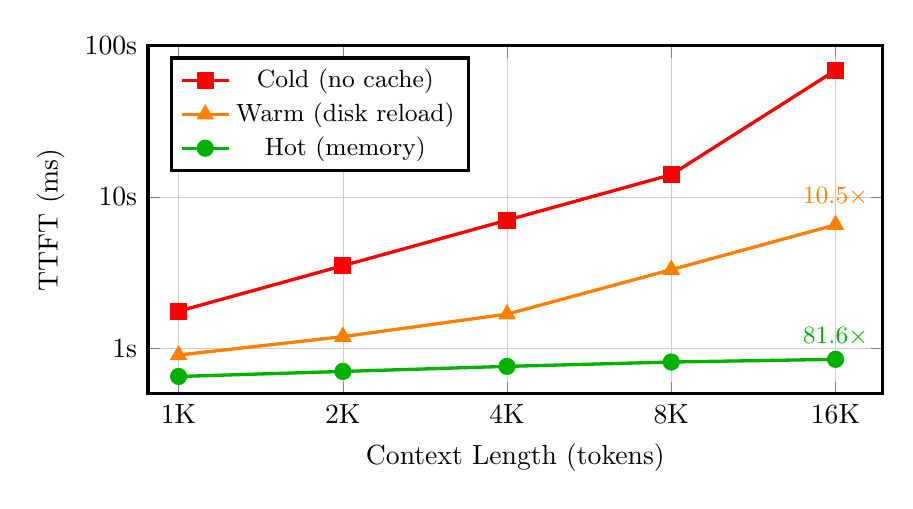
\begin{tikzpicture}
\begin{axis}[
    width=0.9\linewidth,
    height=6cm,
    xlabel={Context Length (tokens)},
    ylabel={TTFT (ms)},
    xmode=log,
    ymode=log,
    log basis x=2,
    log basis y=10,
    xmin=900, xmax=20000,
    ymin=500, ymax=100000,
    xtick={1024,2048,4096,8192,16384},
    xticklabels={1K,2K,4K,8K,16K},
    ytick={1000,10000,100000},
    yticklabels={1s,10s,100s},
    legend pos=north west,
    legend style={font=\small},
    grid=both,
    grid style={line width=.1pt, draw=gray!20},
    major grid style={line width=.2pt,draw=gray!40},
    mark size=2.5pt,
    line width=1.2pt
]

% Cold (no cache) - red
\addplot[color=red, mark=square*] coordinates {
    (1024, 1756)
    (2048, 3512)
    (4096, 7024)
    (8192, 14048)
    (16384, 68898)
};
\addlegendentry{Cold (no cache)}

% Warm (disk reload) - orange
\addplot[color=orange, mark=triangle*] coordinates {
    (1024, 901)
    (2048, 1192)
    (4096, 1680)
    (8192, 3307)
    (16384, 6544)
};
\addlegendentry{Warm (disk reload)}

% Hot (in-memory) - green
\addplot[color=green!70!black, mark=*] coordinates {
    (1024, 650)
    (2048, 702)
    (4096, 758)
    (8192, 810)
    (16384, 844)
};
\addlegendentry{Hot (memory)}

% Annotations
\node[font=\small, text=green!70!black] at (axis cs:16384,1200) {81.6$\times$};
\node[font=\small, text=orange] at (axis cs:16384,10000) {10.5$\times$};

\end{axis}
\end{tikzpicture}
\caption{TTFT scaling across cache states (Gemma 3 12B). Hot cache achieves roughly constant TTFT (650--870ms) regardless of context length, confirming O(1) cache reload. Warm (disk reload) provides 10.5$\times$ speedup at 16K. Cold start exhibits O(n) prefill scaling.}
\label{fig:ttft}
\end{figure}
